\documentclass{article}
\usepackage[utf8]{inputenc}

\usepackage{mathtools}
\usepackage{amsthm}
\usepackage{cancel}
\usepackage{graphicx}

\usepackage{listings}
\usepackage{xcolor}

\usepackage[T1]{fontenc}

\usepackage{graphicx}

\graphicspath{ {../images/} }

\definecolor{codegreen}{rgb}{0,0.6,0}
\definecolor{codegray}{rgb}{0.5,0.5,0.5}
\definecolor{codepurple}{rgb}{0.58,0,0.82}
\definecolor{backcolour}{rgb}{0.95,0.95,0.92}

\lstdefinestyle{mystyle}{
    backgroundcolor=\color{backcolour},   
    commentstyle=\color{codegreen},
    keywordstyle=\color{blue},
    numberstyle=\tiny\color{codegray},
    stringstyle=\color{codegreen},
    basicstyle=\ttfamily\footnotesize,
    breakatwhitespace=false,         
    breaklines=true,                 
    captionpos=b,                    
    keepspaces=true,                 
    numbers=left,                    
    numbersep=5pt,                  
    showspaces=false,                
    showstringspaces=false,
    showtabs=false,                  
    tabsize=2
}

\lstset{style=mystyle}

\title{Obligatorisk oppgave 2, MAT-INF1100, Høst 2020}
\author{Cory Alexander Balaton}
\date{November 2020}

\begin{document}
\maketitle
\newpage

\section*{Task 1}

\subsection*{a}
\lstinputlisting[language=Python]{../Oppg_1/Accel.py}
This is a class that takes the difference of some $y$ values and divides it by the corresponding $x$ values to get an
average acceleration between to points, and plots an acceleration graph. \\

\newpage

\subsection*{b}
\lstinputlisting[language=Python]{../Oppg_1/Distance.py}
This is a class that approximates the area of a curve by using the trapezoidal rule. \\

\newpage

\subsection*{c}
\lstinputlisting[language=Python]{../Oppg_1/TextToList.py}
This class takes a file that contains 2 parameters divided by a comma, converts it to 2 lists, then returns
a list containing the 2 lists. \\

\lstinputlisting[language=Python]{../Oppg_1/main.py}
This is the main program that creates instances of all the classes to create 2 plots. \\

\newpage

\begin{figure}[h]
    \centering
    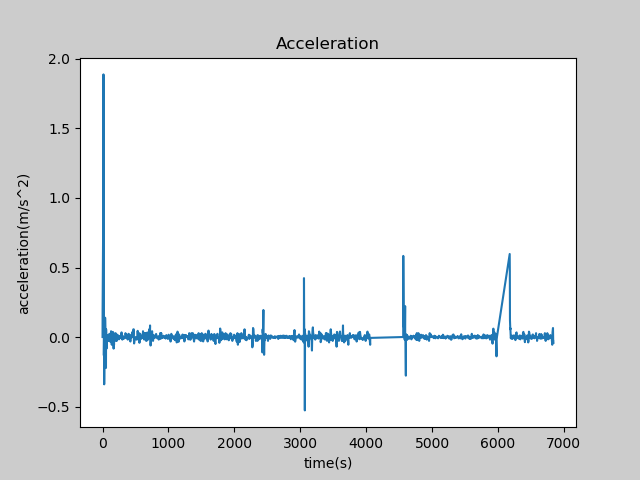
\includegraphics[width=0.6\textwidth]{Accel}
    \caption{Acceleration plot}
    \label{fig:accel}
\end{figure}

\begin{figure}[h]
    \centering
    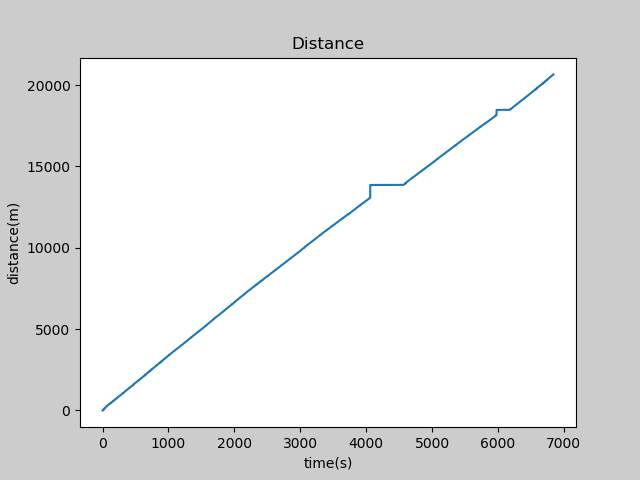
\includegraphics[width=0.6\textwidth]{Distance}
    \caption{Distance plot}
    \label{fig:dist}
\end{figure}

Looking at the Distance plot that was made by the program, it looks like the running session went for a little
bit over 20km.

\newpage

\section*{Task 2}

\subsection*{a}

Under is the original equation:
\begin{equation}
    x' = x(\frac{1}{2} - x), \text{ where } x(0) = 1
\end{equation}

\subsubsection*{Solving the separable differential equation}
Start by separating and then integrating:
\begin{equation}
    \begin{split}
        x' &= x(\frac{1}{2} - x) \\
        \frac{dx}{dt} &= x(\frac{1}{2} - x) \\
        \frac{1}{x(\frac{1}{2} - x)} dx &= 1 dt \\
        \frac{2}{x(1 - 2x)} dx &= 1 dt \\
        \int \frac{2}{x(1 - 2x)} dx &= \int 1 dt \\ %Show the breaking up
        \int \frac{2}{x} + \frac{4}{1-2x} dx &= \int 1 dt \\
        2 \int \frac{1}{x} dx - 2 \int \frac{-2}{1-2x} dx &= \int 1 dt \\
        \text{$u = 1 - 2x$ and $du = -2 dx$} \\
        2 \int \frac{1}{x} dx - 2 \int \frac{1}{u} du &= \int 1 dt \\
        2 \ln|x| - 2 \ln|u| &= t + C \\
    \end{split}
\end{equation}
Then solve the general equation:
\begin{equation}
    \begin{split}
        2 \ln|x| - 2 \ln|u| &= t + C \\
        \ln|x| - \ln|1-2x| &= \frac{t + C}{2} \\
        \ln|\frac{x}{1-2x}| &= \frac{t + C}{2} \\
        |\frac{x}{1-2x}| &= e^{\frac{t + C}{2}}  \\
        |\frac{x}{1-2x}| &= e^{\frac{t}{2}} \cdot e^{\frac{C}{2}}  \\
        \frac{x}{1-2x} &= \pm Ce^{\frac{t}{2}}  \\
        x &= Ce^{\frac{t}{2}} \cdot (1 - 2x) \\
        x &=  Ce^{\frac{t}{2}} - 2x \cdot Ce^{\frac{t}{2}} \\
        x + 2x \cdot Ce^{\frac{t}{2}} &=  Ce^{\frac{t}{2}} \\
        x \cdot (1 + 2 \cdot Ce^{\frac{t}{2}}) &=  Ce^{\frac{t}{2}} \\
        x &= \frac{Ce^{\frac{t}{2}}}{1 + 2 \cdot Ce^{\frac{t}{2}}} \\
        x &= \frac{1}{Ce^{-\frac{t}{2}} + 2} \\
    \end{split}
\end{equation}
Plug in x(0) = 1 to the equation, and solve for C
\begin{equation}
    \begin{split}
        1 &= \frac{1}{Ce^{-\frac{0}{2}} + 2} \\
        1 &= \frac{1}{C + 2} \\
        C + 2 &= 1 \\
        C &= -1
    \end{split}
\end{equation}
Plug in C in equation 3:
\begin{equation}
    \begin{split}
        x = \frac{1}{-1e^{-\frac{t}{2}} + 2} \\
        \underline{\underline{x = -\frac{1}{e^{-\frac{t}{2}} - 2}}} \\
    \end{split}
\end{equation}

\newpage

\subsection*{b \& c}

\lstinputlisting[language=Python]{../Oppg_2/Euler.py}

For task b and c, I created a class Euler that implements the forward euler method, the midpoint euler method,
and a plot method.

\newpage

\lstinputlisting[language=Python]{../Oppg_2/main.py}

This is the main program that uses the Euler class to approximate the curve of the differential equation using
the two method that are available.

\newpage

\begin{figure}[h]
    \centering
    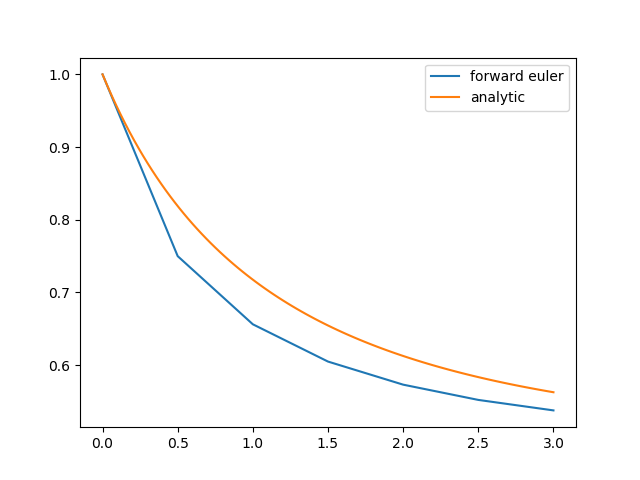
\includegraphics[width=0.6\textwidth]{task_2b}
    \caption{analytical and forward euler plot}
\end{figure}

\begin{figure}[h]
    \centering
    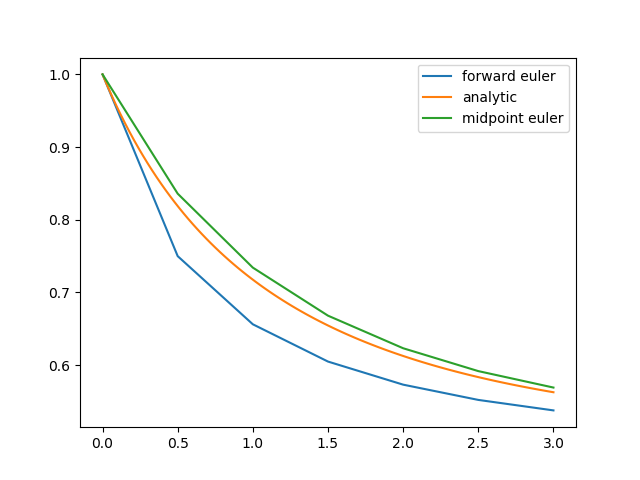
\includegraphics[width=0.6\textwidth]{task_2c}
    \caption{analytical, forward euler, and midpoint euler plot}
\end{figure}

Those are the plots that are created when I run my program, and we can clearly see that the midpoint euler
method is far more precise than the forward euler method, but at a cost of computing power.

\newpage

\subsection*{d}

We know that $x(0) = 1$ is the upper limit for the function if we can prove that $x(t) = \frac{1}{2 - e^{- \frac{t}{2}}}$
is monotonically decreasing (Which looks like is the case in the plots made earlier). \\
The only term that changes in $x(t)$ is $e^{- \frac{t}{2}}$. If we define a function \\
$y(t) = e^{- \frac{t}{2}} = \frac{1}{e^{\frac{t}{2}}}$ and a number $h > 0$ we can see that $y(t + h) \le y(t)$
where $t \ge 0$. \\
We replace $e^{- \frac{t}{2}}$ in $x(t)$ with $y(t)$ so that $x(t) = \frac{1}{2 - y(t)}$. Since we know that $y(t)$
decreases as $t$ gets smaller, the denominator of $x(t)$ will get bigger, which means that $x(t)$ decreases as $t$
gets larger. This means that $x(t)$ is monotonically decreasing when $t \ge 0$. \\ \\

To prove that $x(t) \ge \frac{1}{2}$ for $t \ge 0$, we have to look at what happens when $t \rightarrow \infty$.
\begin{equation}
    \begin{split}
        &\lim_{t \rightarrow \infty} x(t) \\
        = &\lim_{t \rightarrow \infty} \frac{1}{2 - e^{- \frac{t}{2}}} \\
        = &\lim_{t \rightarrow \infty} \frac{1}{2 - e^{- \frac{1}{2}t}} \\
        = &\lim_{t \rightarrow \infty} \frac{1}{2 - e^{- \frac{1}{2}\infty}} \\
        = &\lim_{t \rightarrow \infty} \frac{1}{2 - 0} \\
        = &\frac{1}{2} \\
    \end{split}
\end{equation}
This means that no matter how big $t$ is, $x(t) \ge \frac{1}{2}$. \\ \\

\newpage

This limit also applies for the forward euler method for this equation. this is because $x(t + h) = y(t) + y(t)(\frac{1}{2} - y(t))$ where $h > 0$,
will decrease less and less as $y(x) \rightarrow \frac{1}{2}$. In other words:
\begin{equation}
    \begin{split}
        &\lim_{x \rightarrow \frac{1}{2}}  y(t) + y(t)(\frac{1}{2} - y(t)) \\
        = &\lim_{x \rightarrow \frac{1}{2}}  \frac{1}{2} + \frac{1}{2}(\frac{1}{2} - \frac{1}{2}) \\
        = &\frac{1}{2} + \frac{1}{2}(0) \\
        = &\frac{1}{2} + 0 \\
        = &\frac{1}{2} \\
    \end{split}
\end{equation}
Which means that $x(t) \ge \frac{1}{2}$


\end{document}